\documentclass{standalone}
\usepackage[mode=buildnew]{standalone}
\usepackage{tikz}
\usetikzlibrary{positioning, shapes, arrows}
\begin{document}
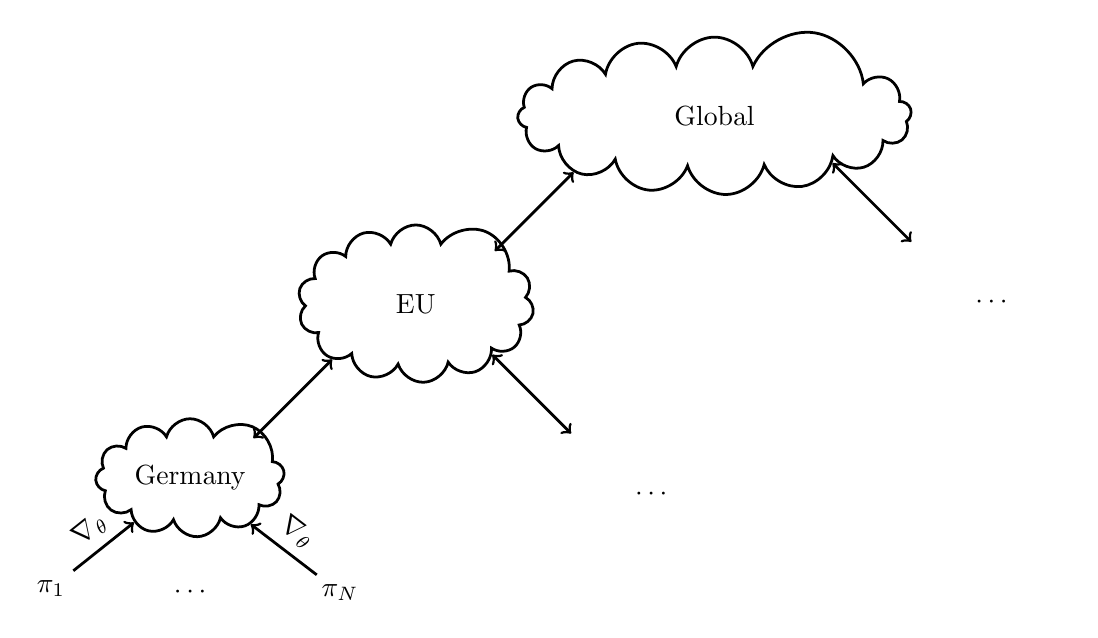
\begin{tikzpicture}
\node[cloud, cloud puffs=15.7, cloud ignores aspect, minimum width=5cm, minimum height=2cm, align=center, draw, line width=1pt] (global) {Global};
\node[minimum width=2cm, minimum height=1.5cm, align=center, below right=of global, , line width=1pt] (region) {$\cdots$};
\node[cloud, cloud puffs=13.7, cloud ignores aspect, minimum width=3cm, minimum height=2cm, align=center, draw, below left=of global, line width=1pt] (eu) {EU};
\node[minimum width=2cm, minimum height=1.5cm, align=center, below right=of eu, , line width=1pt] (eucountry) {$\cdots$};
\node[cloud, cloud puffs=11.7, cloud ignores aspect, minimum width=2cm, minimum height=1.5cm, align=center, draw, below left=of eu, , line width=1pt] (germany) {Germany};
\node[below left=1cm of germany] (pi_11) {$\pi_{1}$};
\node[below=0.5cm of germany] (pi_12) {$\cdots$};
\node[below right=1cm of germany] (pi_1N) {$\pi_{N}$};
\draw[->, line width=1pt] (pi_11) -- (germany) node [midway, above, sloped] {$\nabla_\theta$};
\draw[->, line width=1pt] (pi_1N) -- (germany) node [midway, above, sloped] {$\nabla_\theta$};
\draw[<->, line width=1pt] (germany.north east) -- (eu.south west) {};
\draw[<->, line width=1pt] (eu.north east) -- (global.south west) {};
\draw[<->, line width=1pt] (eu.south east) -- (eucountry.north west) {};
\draw[<->, line width=1pt] (region.north west) -- (global.south east) {};
\end{tikzpicture}
\end{document}